\documentclass[10pt]{article}

\usepackage[margin=1in]{geometry}
\usepackage{times}
\usepackage{microtype}
\usepackage{graphicx}
\usepackage{booktabs}
\usepackage{array}
\usepackage{xcolor}
\usepackage{hyperref}
\usepackage{natbib}
\usepackage{tikz}
\usetikzlibrary{arrows.meta,positioning,shapes.geometric,calc}

\hypersetup{
  colorlinks=true,
  linkcolor=blue!45!black,
  citecolor=blue!45!black,
  urlcolor=blue!45!black
}

\newcommand{\systemname}{SVG Icon Agent}
\newcommand{\rundir}{\texttt{outputs/web/1780452985-591e5896}}

\title{\systemname: A Collaborative LLM-Agent Pipeline for Editable SVG Icon Generation}
\author{
Name: TODO \\
Student ID: TODO \\
Contribution: TODO
}
\date{}

\begin{document}
\maketitle

\begin{abstract}
This report presents \systemname, a generative-AI system that converts a short English icon description into editable SVG artwork through a provider-neutral multi-agent workflow. The code is available at \url{https://github.com/fwar1nben/CG_PJ}. Instead of using a local template generator or a raster image model, the system organizes large-language-model calls into goal management, prompt rewriting, planning, multi-candidate SVG drafting, independent criticism, consensus selection, SVG optimization, validation, failure taxonomy, repair routing, refinement, and memory curation. Deterministic local code is used only as a tool layer for input handling, retrieval over previous local runs, machine-checkable SVG safety checks, PNG export, gallery construction, and logging. The main web experiment in \rundir{} generated a minimal rocket-launch icon with memory enabled and a collaborative workflow. The resulting baseline and refined SVGs were both valid, both scored 100.0 under the current validation rubric, and required zero repair rounds. The result demonstrates a controllable and inspectable agent architecture for graphics-focused generative AI, while also revealing the need for broader quantitative evaluation and stronger perceptual metrics.
\end{abstract}

\section{Introduction}

Text-to-image systems can produce visually rich icons, but their outputs are usually raster images that are hard to edit, inspect, or validate with programmatic constraints. For a computer graphics project, SVG icon generation is a useful alternative target: the output is compact, editable, resolution-independent, and directly tied to vector graphics primitives such as paths, circles, polygons, and gradients. At the same time, SVG is unforgiving. A single malformed tag, unsafe external reference, or over-complicated path can break rendering or make the result difficult to revise.

\systemname{} treats this problem as an agentic generative-AI workflow rather than a one-shot text completion task. Each named Agent calls the configured LLM provider and has a narrow responsibility. Local code does not silently replace failed agents with a handcrafted SVG template. Instead, local tools provide evidence, constraints, export, and logging. This distinction is important for the project goal: the central subject is generative AI practice, while the deterministic layer makes the generated vector artwork inspectable and reproducible.

The system also includes a lightweight web interface. A user can enter a prompt, watch the current Agent node in a directed acyclic workflow graph, inspect rewritten prompts, view retrieved memories, compare selected and optimized SVGs, preview exported PNGs, and read redacted raw LLM responses. This makes the generation process demonstrable rather than hidden behind a single command-line result.

\section{Related Work}

\paragraph{Language-model agents.}
Agentic workflows often combine reasoning, tool use, feedback, and iterative repair. ReAct \citep{yao2023react} showed that language models can interleave reasoning traces with actions, while Reflexion \citep{shinn2023reflexion} showed that verbal feedback can improve later attempts. \systemname{} follows the same high-level idea but specializes it for vector graphics: feedback is converted into SVG-specific critique, failure taxonomy, and repair routes.

\paragraph{Retrieval-augmented generation.}
Retrieval-augmented generation \citep{lewis2020rag} conditions model output on relevant external memory. In this project, memory is local and project-specific. The Memory Retrieval Tool searches prior runs, user feedback, scores, and curated design lessons. The Memory Curator Agent then writes compact reusable records after each run. This avoids using an external dataset while still giving the system experience across repeated prompts.

\paragraph{Agentic visual-design systems.}
Recent visual-design systems such as GenPilot, Paper2Poster, and PosterForest explore multi-agent or tool-augmented workflows for image prompt improvement, scientific-poster generation, and hierarchical poster design \citep{genpilot,paper2poster,posterforest}. \systemname{} is smaller in scope but more graphics-specific: it produces editable SVG source and uses SVG validity, safety, and renderability as first-class signals.

\paragraph{SVG and rendering tools.}
SVG is a W3C vector graphics format \citep{w3csvg2}, with widely used web documentation from MDN \citep{mdnsvg}. The project exports PNG previews using a lightweight local renderer implemented with Pillow \citep{pillowdocs}. The web demo uses Flask \citep{flaskdocs}. LLM calls are made through an OpenAI-compatible provider adapter following OpenRouter's chat-completions API documentation \citep{openrouterdocs}; the Agent names remain provider-neutral.

\section{Method}

\subsection{System Overview}

Figure~\ref{fig:dag} shows the main collaborative workflow. The graph is not purely linear. The candidate generation stage produces multiple candidates, and the semantic and SVG-quality critics evaluate the candidate set as parallel conceptual branches before the selector merges their judgments. The repair stage forms a conditional loop: if validation finds blocking issues, the system diagnoses them, routes the repair strategy, refines the SVG, and validates again.

\begin{figure}[t]
\centering
\resizebox{\linewidth}{!}{
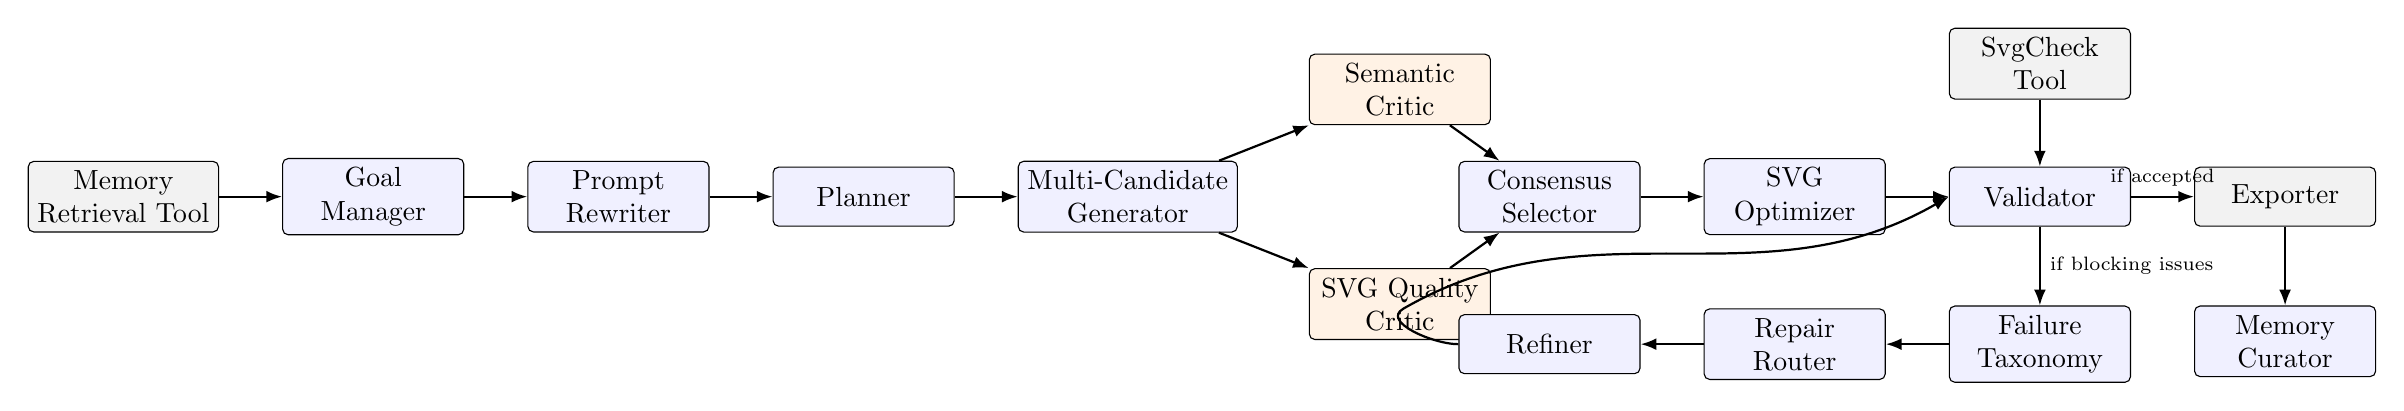
\begin{tikzpicture}[
  node distance=0.75cm and 0.8cm,
  agent/.style={draw, rounded corners=2pt, align=center, minimum width=2.3cm, minimum height=0.75cm, fill=blue!6},
  tool/.style={draw, rounded corners=2pt, align=center, minimum width=2.3cm, minimum height=0.75cm, fill=gray!10},
  critic/.style={draw, rounded corners=2pt, align=center, minimum width=2.3cm, minimum height=0.75cm, fill=orange!10},
  edge/.style={-{Latex[length=2mm]}, thick}
]
\node[tool] (memory) {Memory\\Retrieval Tool};
\node[agent, right=of memory] (goal) {Goal\\Manager};
\node[agent, right=of goal] (rewrite) {Prompt\\Rewriter};
\node[agent, right=of rewrite] (plan) {Planner};
\node[agent, right=of plan] (gen) {Multi-Candidate\\Generator};

\node[critic, above right=0.45cm and 0.9cm of gen] (sem) {Semantic\\Critic};
\node[critic, below right=0.45cm and 0.9cm of gen] (qual) {SVG Quality\\Critic};
\node[agent, right=2.8cm of gen] (selector) {Consensus\\Selector};
\node[agent, right=of selector] (optim) {SVG\\Optimizer};
\node[agent, right=of optim] (valid) {Validator};

\node[agent, below=1.0cm of valid] (tax) {Failure\\Taxonomy};
\node[agent, left=of tax] (route) {Repair\\Router};
\node[agent, left=of route] (refine) {Refiner};
\node[tool, above=0.85cm of valid] (check) {SvgCheck\\Tool};
\node[tool, right=of valid] (export) {Exporter};
\node[agent, below=1.0cm of export] (curator) {Memory\\Curator};

\draw[edge] (memory) -- (goal);
\draw[edge] (goal) -- (rewrite);
\draw[edge] (rewrite) -- (plan);
\draw[edge] (plan) -- (gen);
\draw[edge] (gen) -- (sem);
\draw[edge] (gen) -- (qual);
\draw[edge] (sem) -- (selector);
\draw[edge] (qual) -- (selector);
\draw[edge] (selector) -- (optim);
\draw[edge] (optim) -- (valid);
\draw[edge] (check) -- (valid);
\draw[edge] (valid) -- node[right, font=\scriptsize] {if blocking issues} (tax);
\draw[edge] (tax) -- (route);
\draw[edge] (route) -- (refine);
\draw[edge] (refine.west) to[out=180,in=210] ++(-0.7,0.45) to[out=30,in=210] (valid.west);
\draw[edge] (valid) -- node[above, font=\scriptsize] {if accepted} (export);
\draw[edge] (export) -- (curator);
\end{tikzpicture}
}
\caption{Provider-neutral Agent DAG used by the collaborative workflow. Blue nodes are LLM-backed Agents, gray nodes are deterministic tools, and orange nodes are critic Agents. The repair branch is conditional and only runs when validation reports blocking issues.}
\label{fig:dag}
\end{figure}

\subsection{Agent Roles}

The Goal Manager Agent converts the raw prompt, optional user goal, and retrieved memories into an explicit objective, visual requirements, constraints, acceptance criteria, style preferences, and avoid patterns. The Prompt Rewriter Agent then expands the raw request into an SVG-focused prompt while avoiding unnecessary hard-coded color choices. The Planner Agent produces a structured icon plan that downstream Agents can consume.

The Multi-Candidate Generator Agent produces several complete SVG drafts. The Semantic Critic Agent evaluates prompt alignment, recognizability, and small-icon readability. The SVG Quality Critic Agent evaluates editability, safety, primitive simplicity, and rendering risk using local tool evidence. The Consensus Selector Agent chooses the best candidate and writes an explicit repair brief.

The SVG Optimizer Agent receives the selected candidate, critic reports, selector rationale, local tool checks, and optional human feedback. It returns an optimized SVG that becomes the baseline artifact. This design makes ``baseline'' stronger than a raw first draft: it is the result of collaboration before validation.

The Validator Agent judges the optimized SVG using both semantic criteria and local machine-checkable evidence. If no blocking issue is found, the refined artifact can equal the baseline and the repair branch is skipped. If blocking issues exist, the Failure Taxonomy Agent classifies issue types, root causes, evidence, priority, and repair goals. The Repair Router Agent then converts this diagnosis into ordered actions and a concise Refiner brief. The Refiner Agent must return a complete repaired SVG, which is validated again.

Finally, the Memory Curator Agent summarizes the run into a short reusable memory record. This memory contains design strategies, failure patterns, user feedback, score, and tags. Future runs can retrieve it through the local Memory Retrieval Tool.

\subsection{Local Tools and Safety Boundary}

The local SvgCheckTool parses SVG, checks canvas and viewBox requirements, rejects unsafe tags and external references, estimates primitive count, and records renderability risks. It is deliberately not named an Agent because it does not call the model. The exporter writes selected, baseline, and refined SVG artifacts, renders PNG previews, builds an HTML gallery, and records metrics and LLM traces. Raw LLM responses are saved in redacted logs so that API keys and secrets are not stored.

\section{Experimental Results}

\subsection{Data Source}

The primary evidence comes from the latest complete web run at \rundir. The user prompt was:
\begin{quote}
\small
\texttt{a minimal rocket launch icon with a dynamic flame}
\end{quote}
The run used the collaborative workflow, enabled memory retrieval with top-$k=3$, and recorded the model identifier \texttt{deepseek/deepseek-v4-flash} in the trace. No public dataset was used; the result is based on a self-authored prompt and local historical run memory.

\subsection{Goal and Memory Context}

The Goal Manager Agent converted the short prompt into a more explicit target: a 256-by-256 SVG app-style rocket launch icon with a centered upright rocket body, pointed nose cone, small fins, layered sweeping flame curves, balanced whitespace, and small-size legibility. Retrieved memories were highly relevant previous rocket runs. They suggested success patterns such as a centered upright rocket, layered flame curves, and warm flame gradients, and they preserved prior human feedback to simplify the rocket window into a single filled circle.

\begin{table}[t]
\centering
\caption{Main web-run configuration and outcome from \rundir.}
\label{tab:main}
\begin{tabular}{ll}
\toprule
Field & Value \\
\midrule
Workflow & Collaborative \\
Prompt source & Web manual input \\
Model recorded in trace & \texttt{deepseek/deepseek-v4-flash} \\
Memory enabled & Yes, top-$k=3$ \\
Candidate count & 3 \\
Selected candidate & Candidate 2 \\
Baseline valid & 1 / 1 \\
Refined valid & 1 / 1 \\
Baseline score & 100.0 \\
Refined score & 100.0 \\
Score delta & 0.0 \\
Repair rounds & 0 \\
\bottomrule
\end{tabular}
\end{table}

\subsection{Candidate Competition}

Table~\ref{tab:candidates} shows the candidate-level evidence recorded in \texttt{llm\_trace.json}. All three candidates passed the deterministic SVG tool score, but the critic Agents disagreed on visual strengths. Candidate 2 received the highest semantic score, while Candidate 3 received the highest SVG-quality critic score. The Consensus Selector chose Candidate 2 because it best balanced prompt alignment, dynamic flame curves, and small-icon legibility. Its repair brief recommended enlarging the fins and adjusting the flame boundary.

\begin{table}[t]
\centering
\caption{Candidate competition recorded by the collaborative workflow.}
\label{tab:candidates}
\begin{tabular}{lccc}
\toprule
Candidate & Tool score & Semantic critic & SVG-quality critic \\
\midrule
Candidate 1 & 100 & 85 & 90 \\
Candidate 2 & 100 & 92 & 88 \\
Candidate 3 & 100 & 70 & 95 \\
\bottomrule
\end{tabular}
\end{table}

\subsection{Qualitative Result}

Figure~\ref{fig:rocket} compares the optimized baseline PNG and final refined PNG. Since the Validator Agent found no blocking issues, the failure-taxonomy, repair-router, and refiner branch did not run for this case. Therefore, the refined score remained equal to the baseline score. This is a positive outcome for the example, but it also means this run should not be used as evidence that the repair router improves failing SVGs. It only shows that the system can skip repair when validation accepts the optimized result.

\begin{figure}[t]
\centering
\begin{minipage}{0.42\linewidth}
\centering

\includegraphics[width=0.75\linewidth]{figures/rocket_baseline.png}\\
\small Baseline after SVG Optimizer
\end{minipage}
\hfill
\begin{minipage}{0.42\linewidth}
\centering

\includegraphics[width=0.75\linewidth]{figures/rocket_refined.png}\\
\small Refined output
\end{minipage}
\caption{Qualitative result from the latest complete web run. The final image equals the validated optimized baseline because no repair round was required.}
\label{fig:rocket}
\end{figure}

\subsection{Discussion}

The experiment demonstrates four important properties. First, the workflow is inspectable: the run records the rewritten prompt, generation goal, retrieved memories, candidate scores, selector rationale, optimizer feedback sources, validation result, and usage data. Second, the design separates LLM-backed Agents from deterministic tools, making it clear which modules are generative and which modules enforce mechanical constraints. Third, the system supports memory-based iteration: previous human feedback and successful design patterns were retrieved and reused. Fourth, the web UI makes the DAG visible, which is useful for a course demo because users can see which Agent is active rather than waiting for a black-box response.

The current evidence is still limited. The main web run contains one prompt, and its repair branch was skipped. Earlier root-level batch artifacts include more prompts, but their metrics and traces are not fully aligned in the current output snapshot, so they are not used as the primary quantitative claim. A stronger final evaluation should rerun the complete prompt set through the current collaborative workflow, include intentionally difficult prompts that trigger repair, and compare against the single-workflow ablation.

\section{Conclusion}

\systemname{} is a compact generative-AI practice project for editable vector icon generation. Its main contribution is not a new SVG renderer, but an inspectable multi-agent organization around goal management, memory retrieval, prompt rewriting, candidate competition, critique, optimization, validation, failure diagnosis, repair routing, and memory curation. The latest web run produced a valid high-scoring rocket icon and preserved detailed traces for every active Agent. Future work should expand the evaluation set, add perceptual visual metrics, study human preference ratings, and test whether the Failure Taxonomy and Repair Router Agents improve recovery on malformed or semantically weak SVG generations.

\bibliographystyle{plainnat}
\bibliography{references}

\end{document}
